%!TEX TS-program = pdflatex
%!TEX root = progetto_finale.tex
%!TEX encoding = UTF-8 Unicode

\chapter{Implementazione}

Il linguaggio scelto per l'implementazione del progetto è Erlang. Esso è stato selezionato per diversi motivi tra cui: fornisce nativamente il supporto alla gestione di messaggi e scambio di essi tra diverse entità; permette di creare in poche righe di codice diversi beam a cui poter richiedere dei servizi; grazie alla libreria ``gen\_statem'' è possibile creare facilmente gli automi e le interazioni fra essi.

In questo progetto non utilizzate piattaforme esterne di alcun genere poiché si assume che l'autenticazione tra utente e applicazione per il servizio sia già stata effettuata.

Essendo un'architettura peer to peer, non è necessaria alcuna piattaforma a parte l'autenticazione cliente - servizio.

\section{Generazione dell'ambiente virtuale}
Il problema della modellazione di una città è stato risolto con un grafo pesato connesso non orientato: si assume che se due nodi sono connessi è perché vi è una strada tra di essi ed è bidirezionale. Il peso indica quanto costa attraversarla. 

\subsection{Entità presenti}
\subsection{Automi}
Per l'implementazione degli automi è stata utilizzato il behavior erlang "gen\_statem", il quale semplifica la costruzione di macchine a stati finiti guidate da eventi. Questo behavior è un framework con numerose primitive riguardanti questi costrutti: invio e ricezione di eventi sincroni o asincroni, impostazione di timer e molto altro. Gli schemi degli automi mostrati in ... sono stati implementati in modo relativamente veloce potendosi concentrare quasi esclusivamente sulla logica del loro funzionamento piuttosto che sui dettagli implementativi, nascosti appunto dal suddetto framework. 
Qui di seguito si riporta un link alla documentazione ufficiale del framework: ...
Si immagina che i diversi nodi siano posizionati all'interno di un piano cartesiano, pertanto possiedono delle coordinate che ne indicano la posizione. Questo permette di capire la distanza tra di essi e quindi se diverse entità riescono a comunicare tra di loro.

\subsection{Componenti del grafo}
Ogni nodo del grafo possiede quattro proprietà:
\begin{itemize}
	\item attributo nome: generato del tipo ``aa'', ``ab'', ``ac'', ... incrementale per ogni nodo.
	\item attributo id: numero incrementale per ogni nodo a partire da 0. Utilizzato per la definizione del grafo della città.
	\item Coordinate X e Y: definiscono la posizione del nodo all'interno del piano cartesiano rappresentante la città.
\end{itemize}

Gli automi implementati rispettano fedelmente gli schemi mostrati ..., fatta eccezione per alcune mancanze e piccole modifiche che verranno ora elencate

\begin{itemize}
	\item Negli schemi progettuali si mostrava come la comunicazione fra automi interni a un'automobile non avvenisse mai in modo diretto, infatti l'ascoltatore del mezzo si comportava da proxy fra i due automi. Questa scelta progettuale è stata rivista in fase di implementazione, infatti si è ritenuto più veloce permettere una comunicazione diretta, ottenendo anche un codice più snello, pulito e dal comportamento più chiaro. 
	La comunicazione fra un automa interno al veicolo e un automa esterno, come per esempio fra l'automa dell'elezione e l'applicazione utente, avviene tuttavia usando l'ascoltatore come proxy, il quale infatti è l'interfaccia col mondo esterno per un veicolo. Questo ha permesso di diminuire le dipendeze fra i diversi automi: un automa esterno al mezzo deve conoscere soltanto l'ascoltatore per poter comunicare con il veicolo e tutte le sue istanze.
	\item come descritto sopra in ... non è stato aggiunto il cambiamento della topologia cittadina, pertanto gli automi non presentano gli eventi correlati.
	\item Negli schemi progettuali erano stati inseriti molti stati che non presentano una controparte nel codice, questi erano stati definiti in fase di progettazione per chiarire le idee sui comportamenti degli automi, o per rendere gli schemi più espressivi, ma non si è ritenuto utile o conveniente inserirli nella loro implementazione. Il comportamento degli automi non è stato tuttavia intaccato dall'eliminazione di questi stati. 
	\item Similmente agli stati, alcuni eventi riportati negli schemi progettuali non presentano una controparte "esatta" negli automi, nel senso che i nomi di questi eventi sono stati ridefiniti in fase implementativa trovando alternative più espressive o, in generale, migliori per le esigenze del codice. Anche in questo caso il comportamento non è stato intaccato ed è possibile trovare un isomorfirmo fra i nomi degli eventi inseriti negli schemi e quelli inseriti nel codice.
\end{itemize}

\subsubsection{Struttura generale}
I diversi automi implementati presentano tutti uno stato interno, inteso come una propria memoria che varia durante l'esecuzione, ed è importante non confondersi con lo stato della macchina a stati finiti, la similitudine fra i due termini si presta a diversi fraintendimenti e d'ora in poi si userà il termine "memoria" per indicare lo stato con questa accezione. La memoria di ogni automa è stata modellata definendo un record specifico, il quale aggrega tutti i dati necessari.
 
Il codice dei diversi automi è organizzato con una struttura molto simile che si può schematizzare in queste 4 sezioni:

\begin{enumerate}
	\item Codice per l'importazione di metodi da moduli esterni,importazioni di costanti definite esternamente, esportazione di metodi, definizione di costanti utilizzate solo localmente.
	\item definizione del record specifico per l'automa: secondo quanto detto ne modella la sua memoria.
	\item elenco dell'API dell'automa: inteso come le funzionalità della sua interfaccia, esportate per essere usate da altri automi.
	\item funzioni dell'automa: ricalcano gli stati dell'automa e le possibili possibili comportamenti a seguito della ricezione dei vari eventi, la logica dell'automa è raccolta in questa sezione
	\item funzioni interne: usate localmente.
\end{enumerate}

dwdqdw

\subsection{Fornitori di servizi}
Per quanto riguarda gli archi, essi posseggono tre proprietà:
\begin{itemize}
	\item ID\_Nodo\_1 - ID\_Nodo\_2: indica quali nodi collega.
	\item Peso: indica il peso dell'arco, calcolato in funzione della distanza tra i nodi che collega l'arco.
\end{itemize}

Infine vengono selezionati alcuni nodi tra quelli del grafo che conterranno le colonnine di ricarica. Per far questo è stato applicato il seguente algoritmo:
\begin{enumerate}
	\item In base al numero totale delle colonnine, il piano cartesiano viene suddiviso in parti uguali.
	\item Selezione di un nodo casuale all'interno della parte creata a cui assegnare la colonnina.
\end{enumerate}

\subsection{Parametri per la generazione}
Il linguaggio utilizzato per la generazione della città è python. All'interno del file ``map\_generator'' è possibile impostare i diversi parametri per la generazione della città, vale a dire:
\begin{itemize}
\item WEIGHT\_MIN: Peso minimo degli archi.
\item WEIGHT\_MAX:  Peso massimo degli archi.
\item TOTAL\_NODES: Totale numero di nodi del grafo.
\item TOTAL\_EDGES:  Totale numero di archi del grafo.
\item TOTAL\_CHARGING\_COLS:  Totale numero delle colonnine di ricarica nel grafo.
\item CARTESIAN\_SIDE:  Lato del quadrato cartesiano utilizzato per la mappa.
\end{itemize}

Per quanto riguarda il numero di colonnine, esso non è garantito essere rispettato per il seguente motivo: come spiegato precedentemente, l'algoritmo utilizzato suddivide il piano in parti uguali ma potrebbe capitare nel caso esse siano piccole che non vi sia alcun nodo all'interno. Dato che in ogni zona è presente al più una colonnina, può capitare che non siano presenti zone con nodi liberi a cui assegnare le rimanenti.

\subsection{File generati}
Lo script in python crea cinque file:
\begin{itemize}
	\item ``map.pdf'': I dati generati per il grafo vengono esportati nel formato dot e da esso viene generato questo file al cui interno è presente una rappresentazione visuale del grafo: sono presenti i nodi con le proprietà descritte precedentemente e gli archi con delle etichette rappresentanti il loro peso. Un esempio del pdf prodotto è l'immagine \ref{fig:esempio_citta_dot}.
	\item ``map.png'': Rappresentazione visuale delle posizioni dei nodi all'interno del piano cartesiano. I nodi colorati di rosso sono quelli contenenti le colonnine di ricarica. Un esempio del png prodotto è l'immagine \ref{fig:esempio_citta_png}.
	\item ``city\_map\_nodes.dat'': file testuale contenente i dati dei nodi formattati in modo da essere compatibili con la struttura creata in erlang. Un esempio è il seguente:
	\begin{lstlisting}
		10
		a 0 1 4
		b 1 2 12
		c 2 3 12
		d 3 3 16
		e 4 5 2
		...
	\end{lstlisting}
	\item ``city\_map\_graph.dat'': file testuale contenente i dati del grafo formattato in modo da essere compatibile con la libreria utilizzata in erlang. Un esempio è il seguente:
	\begin{lstlisting}
		10 30 undirected d
		6 0 17
		0 1 12
		1 8 18
		8 4 20
		4 7 14
		7 3 21
		3 9 18
		...
	\end{lstlisting}
	\item ``city\_map\_charging\_cols.dat'': file testuale contenente i dati dei nodi delle colonnine. Essi sono formattati in modo da essere compatibili con la struttura creata in erlang. Lo stile è il medesimo del file ``city\_map\_nodes.dat''.
	
\end{itemize}

\begin{figure}[htbp]
	\centering
	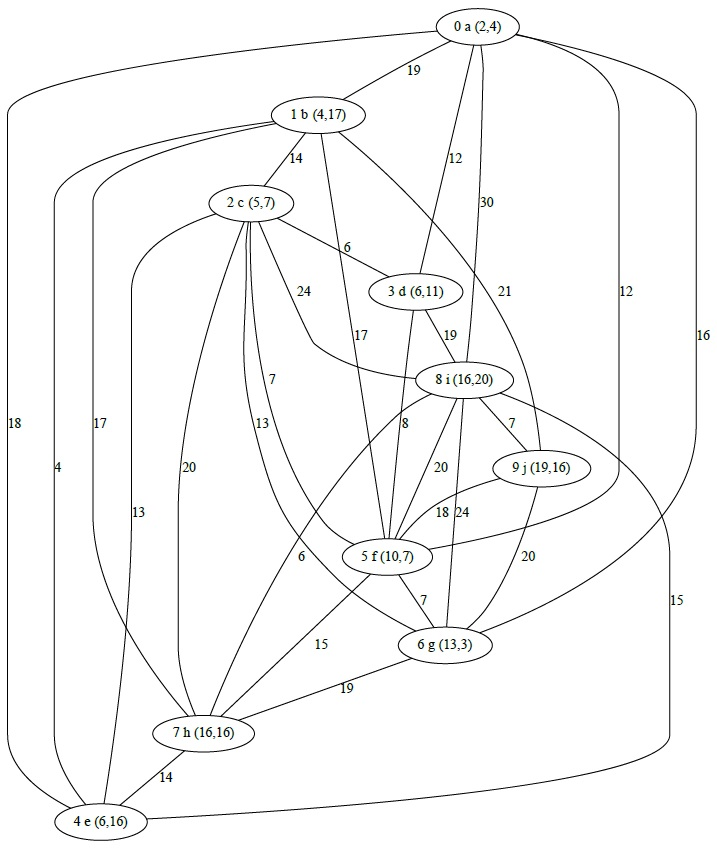
\includegraphics[width=14cm]{esempio_citta_dot.jpg}
	\caption{Esempio di grafo utilizzato per la simulazione della città.}
	\label{fig:esempio_citta_dot}
\end{figure}


\begin{figure}[htbp]
	\centering
	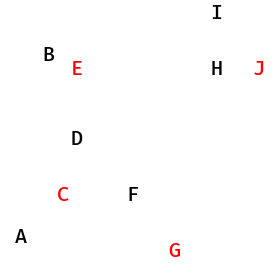
\includegraphics[width=8cm]{esempio_citta_png.jpg}
	\caption{Esempio del posizionamento dei nodi all'interno della città.}
	\label{fig:esempio_citta_png}
\end{figure}


\section{Entità presenti}

\section{Fornitori di servizi}

\section{Automa Elezione}

\section{Interazione tra i diversi moduli}




Details about the implementation: every choice about platforms, languages, software/hardware, middlewares, which has not been decided in the requirements.
Important choices about implementation should be described here; e.g., peculiar data structures.